\chapter{Analysis}
\label{analysis}
\null\qquad After the set of parallelisability metrics has been devised and proposed (see chapter \ref{metrics}) and a working framework for metrics research and analysis has been implemented and set (chapter \ref{ppar-tool} describes developed PPar tool), software source code parallelisability metric values can be gathered and analysed. This analysis task in not that trivial. There is, principally, an unlimited number of ways in which this data can be visualized, interpreted and processed. This chapter describes taken analysis approaches and presents findings in the report.\newline
\null\qquad Table \ref{analysis-data-table} below presents the data, used for analysis. This data has been extracted from NAS parallel benchmarks (see chapter \ref{benchmarks}) and transformed into tabular format.
\begin{figure}[htb]
\centering
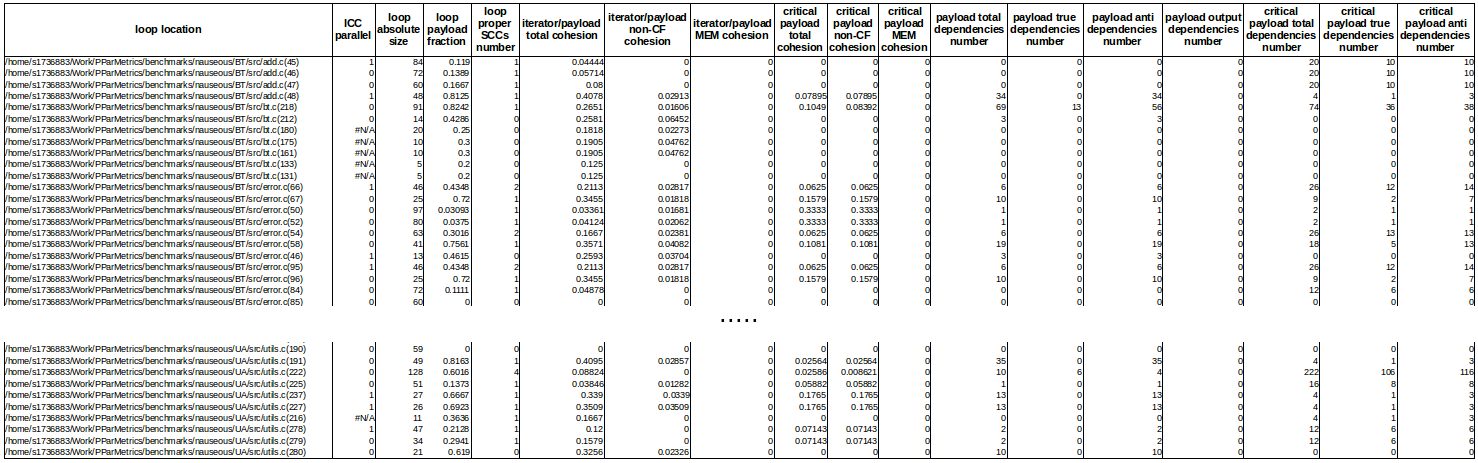
\includegraphics[width=\linewidth]{figs/metrics-table.png}
\caption{Analysis input table with computed metrics and ICC parallelizability classification labels.}
\label{analysis-data-table}
\end{figure} \newline
\null\qquad This data is, essentially, a set of loops found in NAS benchmarks. For every single loop a vector of metrics (loop features) has been computed. All loops have passed through Intel C/C++ compiler parallelisability analyses and have been classified (labelled) as parallelizible or not. ICC compiler plays a role of an expert in this project. The table \ref{analysis-data-table} contains around 1400 loops with 13-dimensional feature vector for each.\newline 
\null\qquad This dataset has been analysed in several ways. First, the collected data has been visualized to see if there are any obvious correlations between loop parallelisability and metric values. Section \ref{analysis-data-interpretation-and-visualization} presents these visualizations and describes all found corerlations. This visualization has been done for every single metric (see subsection \ref{analysis-single-metrics-vs-parallelizability}) as well as for the whole set of metrics altogether (see subsection \ref{analysis-data-clustering-analysis}). To visualize the whole combined set of metrics Principal Component Analysis (PCA) and clustering techniques have been used. Section \ref{analysis-manual-analysis} supplements these visualizations with some manually derived insights into benchmarks source code. \newline 
\null\qquad As another mean of parallelizability metrics examination, statistical analysis techniques have been applied to the data. Loop metrics have been viewed as machine learning features in the context of loop parallelizability classification problem. Standard state-of-the-art  machine learning techniques (such as Support Vector Machines (SVM), desicion trees and neural network based Multi-layer Perceptron (MLP) scikit learn algorithm) have been applied to the data and all prediction errors have been compared against random predictor. Section \ref{analysis-statistical-analysis} presents a report on this.\newline
\null\qquad There has already been an attempt to apply statistical analysis techniques to see how software quality metrics, such as cyclomatic complexity \ref{background-cyclomatic-complexity} and Halstead's software science measures \ref{background-halsteads-measures} behave on Mozilla Firefox browser and LLVM compiler components library open source codes \cite{source-code-quality-classification-paper}. Authors applied k-means clustering and got 3 clusters of software quality metric values for subroutines. But there were no classifications attached to the input data and no correlations have been examined. There could easily be subroutines of different software quality grades in the same cluster. \newline
\null\qquad All results have been derived thanks to Python programming language and its packages: pandas \cite{python-lib-pandas}, matplotlib \cite{python-matplotlib} and scikit-learn \cite{python-lib-scikit-learn}. 

\section{Analyses preparation phase}
\label{analysis-preparation-phase}
\qquad Before we move onto the actual description of gathered results, there is a need to describe some preparatory data preprocessing procedures, which have been used throughout all analysis stages. \newline  
\null\qquad As it turned out, there are some outliers in the collected data that distort the final result. For example, figure \ref{outliers-filtering} shows the plot of payload total dependencies number metric values on all NAS benchmark loops. The plot on the left shows metric values dispersion before outliers elimination. It can be seen that there is a non-parallelizible (red dot) loop with almost 12000 dependencies in the payload which seriously shifts mean metric values for parallelizible and non-parallelizible subsets to the point of correlation inversion. Generally, it makes sense that the more dependencies we have in the payload, the harder it has to be to parallelize the loop. And it is seen from the whole dataset that loops with really high dependencies numbers have not been parallelized by the ICC compiler. But for majority of loops, encountered in NAS benchmarks, this tendency does not take place. Right plot contains only those loops, which have metric values withing 3 standard deviations from the mean. Here ICC parallelization ability does not really correlate with the amount of dependencies in the payload of the loop. The total number of dependencies in the payload of a loop is not the only metric, where we have some outliers. Similar filtering measures have been taken for all metrics.   
\begin{figure}[h]
\centering
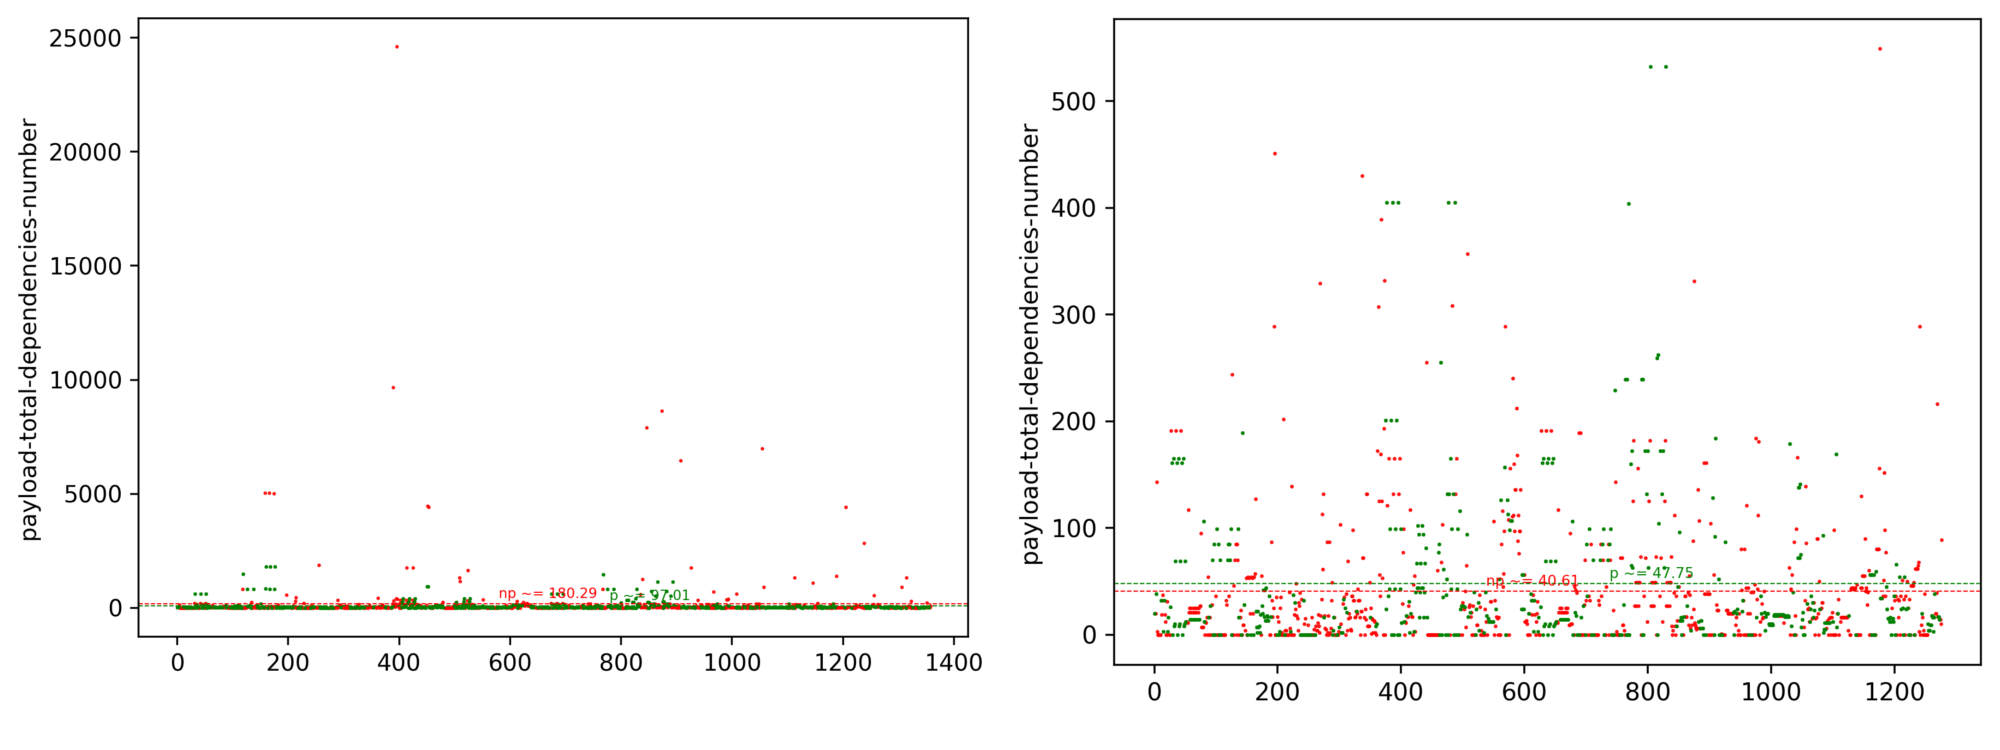
\includegraphics[width=\linewidth]{figs/outliers-filtering.png}
\caption{Distribution of total dependencies number metric values on all NAS benchmark loops before and after elimination of all cases beyond 3 standard deviations from the mean.}
\label{outliers-filtering}
\end{figure} \newline 
\null\qquad There was also a need to normalize the data before application of Principal Component Analysis (PCA) algorithm, in order to make a better graphical visualization.

\section{Data interpretation and visualization}
\label{analysis-data-interpretation-and-visualization}
\qquad This section presents different attempts to find any patterns and correlations in the data from the table \ref{analysis-data-table}. First, every single metric (out of all 13 presented in the table metrics) has been examined alone. Section \ref{analysis-single-metrics-vs-parallelizability} contains all results of single metric parallelizability analysis. Then, the set of metrics has been considered altogether as a whole (as points in 13-dimensional space) in order to find any structural patterns they form. Principal Component Analysis and k-means clustering have been used for that task. Results are presented in subsection \ref{analysis-data-clustering-analysis}.
\subsection{Single loop metrics vs loop parallelisability analysis}
\label{analysis-single-metrics-vs-parallelizability}
\qquad The layout of this section corresponds to that of section \ref{metrics-metric-groups}, which describes proposed groups of software parallelizability metrics. Subsections below present studies of their parallelizability correlation.
\subsubsection{Loop proportion metrics}
\label{analysis-loop-proportion-metrics}
\qquad Figures \ref{loop-proportions-0} and \ref{loop-proportions-1} present scattered plots of all loop proportion metric values, gathered on NAS benchmark loops. Numbers on vertical axes represent metric values, values on horizontal axes represent particular loops in the set. Dashed horizontal lines, crossing plots, represent mean values for subsets of parallelizible (green) and non-parallelizible (red) loops. Numbers show how many dots lie above and below mean values for red and green subsets. All outliers lying beyond 3 standard deviations have been filtered (see section \ref{analysis-preparation-phase}). 
\begin{figure}[htb]
\centering
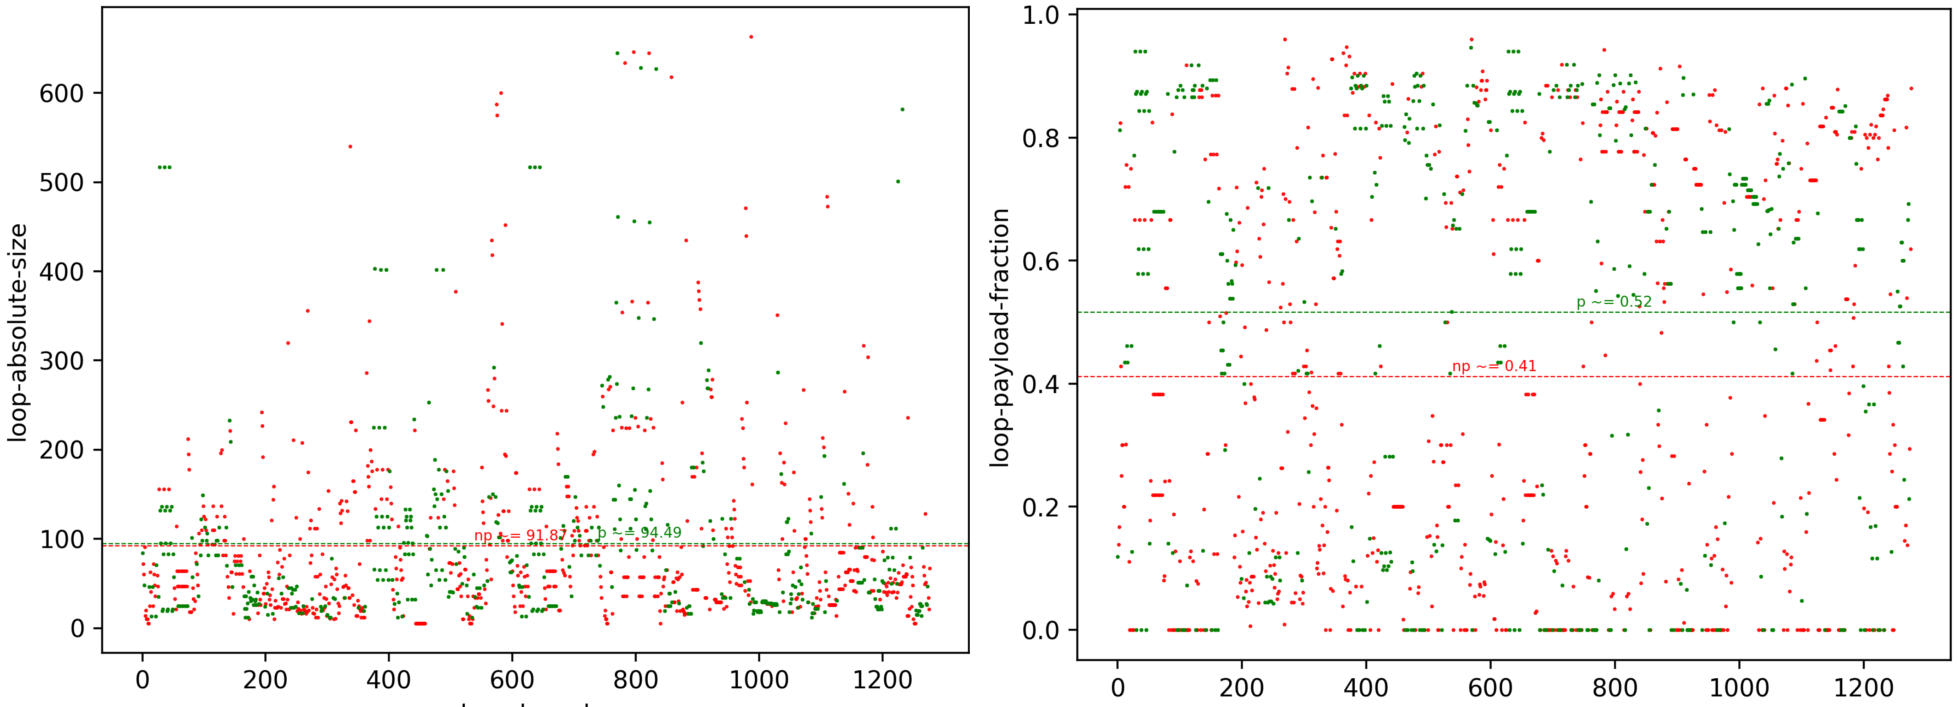
\includegraphics[width=\linewidth]{figs/loop-proportions-0.png}
\caption{\textit{Loop absolute size} metric on the left and \textit{loop payload fraction} metric on the right. Red and green dots represent loops, which have not/have been parallelized by ICC compiler correspondingly. Dashed lines show mean metric values for red and green subsets correspondingly.}
\label{loop-proportions-0}
\end{figure}
\begin{figure}[htb]
\centering
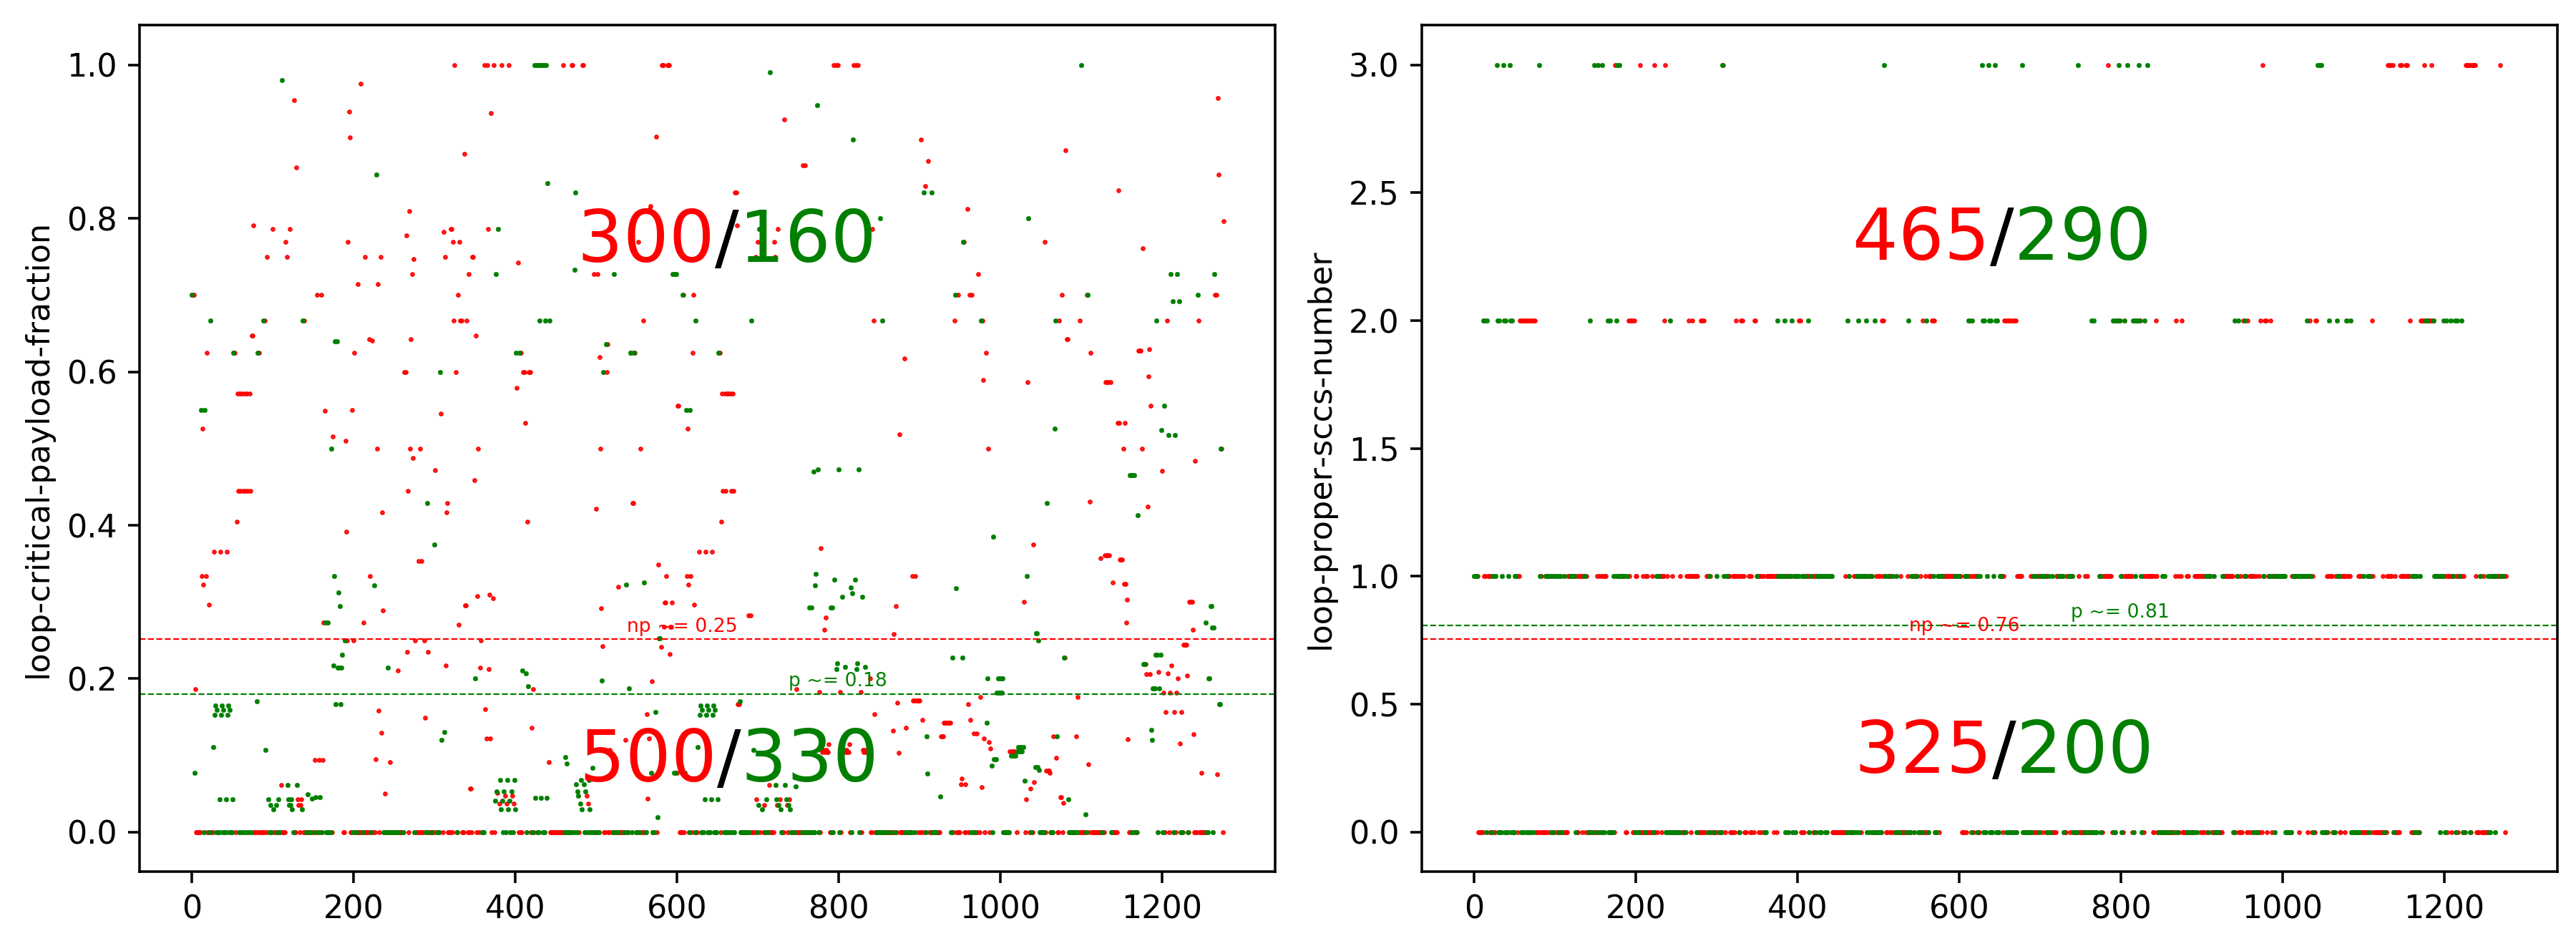
\includegraphics[width=\linewidth]{figs/loop-proportions-1.png}
\caption{\textit{Loop critical payload fraction} metric on the left and \textit{loop proper SCCs number} metric on the right. Analogous to \ref{loop-proportions-0} figure.}
\label{loop-proportions-1}
\end{figure} \newline
\null\qquad As it can be seen from the plots, \textit{loop absolute size} metric values do not really correlate with ICC parallelization ability. Mean values of that metric are almost identical, ~91,87 and 94,49 LLVM-IR instructions, for non-parallelizible and parallelizible loop subsets correspondingly. Red and green dots are scattered above and below mean value lines in similar proportions (210/580$\approx$0,36 and 120/360$\approx$0,33) - majority of NAS loops are smaller than 90 LLVM-IR instructions.\newline
\null\qquad It must be clear from the nature of this metric, that size by itself does not prohibit loop parallelization. There might be a big loop with no cross-iteration dependencies, which must have a big portion of parallelism and should bring huge overall performance gains with its parallelization. And vice versa, there might be a small loop with cross-iteration dependency, which is non-parallelizible.\newline
\null\qquad There is a pretty noticeable correlation between loop parallelisability and values of \textit{loop payload fraction} metric. Green dots are scattered predominantly at the top of the plot. Dot numbers above and below mean lines are in inverse proportionality for red and greed dot subsets (370/420$\approx$0,88\textless 1 and 300/190$\approx$1,58\textgreater 1).  The bigger the payload of a loop in comparison with its iterator, the more seducing this loop for compiler to parallelize. Bigger payloads bring better performance gains with parallelization. Another consideration might also be applied here. Bigger iterators are common for loops, which, for example, perform traversal of more complex data structures like linked-lists or alike. Such loops contain memory operations linking iterator and payload - \textit{iterator payload memory cohesion} metric should be non zero for such loops. Unfortunately, there are no such loops in NAS benchmark set and the latter metric has been excluded from consideration at all.\newline 
\null\qquad Despite the fact that \textit{loop proper SCCs number} metric does not correlate with loop parallelizability that much, another metric of the same essense shows pretty good correlations. \textit{Loop critical payload fraction} metric can be used to judge about loop parallelizability. Connection between this metric and parallelizability property follows just out of common sense. Critical payload parts represent strongly connected components with more than one instructions. There are PDG graph loops with forward and back edges inside such SCCs. Usually it happens when two memory instructions reference the same location on different (or the same) loop iterations and introduce 2 inverse-directed edges with anti and true dependencies. Such critical loop payload parts introduce actual parallelization constraints. The left plot in the figure \ref{loop-proportions-1} illustrates this connection. The bigger the critical component in the payload, the harder it is to parallelize the loop.
\subsubsection{Loop Dependence Metrics}
\label{analysis-loop-dependence-metrics}
\qquad Figures \ref{loop-dependencies-number-0}, \ref{loop-dependencies-number-1} and \ref{loop-dependencies-number-2} present plots of loop dependencies number metric values. These metrics do not seem to be particularly reliable, when it comes to judging about loop parallelizability. Due to this reason the two latter plots have been moved into appendix section.\newline  
\begin{figure}[h]
\centering
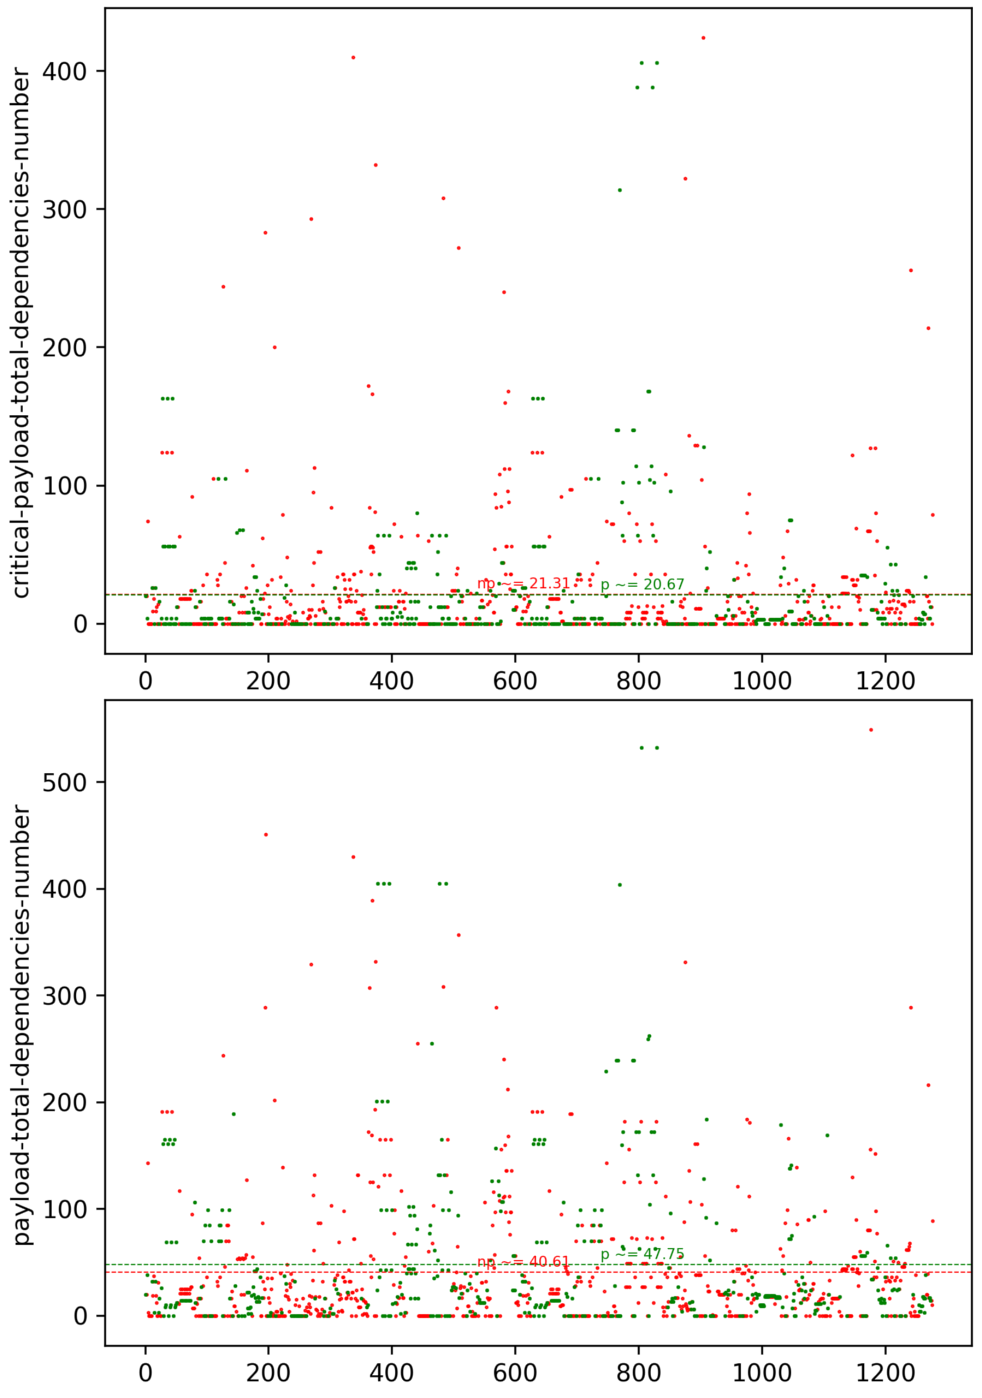
\includegraphics[width=\linewidth]{figs/loop-dependencies-number-0.png}
\caption{\textit{Critical payload dependencies number} metric on the left and \textit{total payload dependencies number} metric on the right. Red and green dots represent loops, which have not/have been parallelized by ICC compiler correspondingly. The other 4 metrics show similar behavior and have been moved into appendix section (see plots \ref{loop-dependencies-number-1} and \ref{loop-dependencies-number-2}).}
\label{loop-dependencies-number-0}
\end{figure}
\null\qquad As it can be seen from the figures, distributions of parallelizible and non-parallelizible (green and red) dots are quite uniform throughout the whole spectrum of metric values. Mean metric values on green and red subsets are also quite close to each other. In cases, where they differ, that difference dissappears with addition of excluded outliers to consideration. Even for loops with a huge total dependencies number either in critical part or in the whole loop payload, ICC compiler sometimes is able to generate a parallel version. All these points show that loop dependencies number metrics cannot be used alone for loop parallelizability analysis.    
\subsubsection{Loop Cohesion Metrics}
\label{analysis-loop-cohesion-metrics}
\qquad Loop cohesion metrics have been described in section \ref{metrics-loop-cohesion-metrics}. Figures \ref{loop-cohesion-0} and \ref{loop-cohesion-1} present plots of loop cohesion metric values on the set of NAS benchmark loops (roughly 1300 loops).\newline    
\begin{figure}[h]
\centering
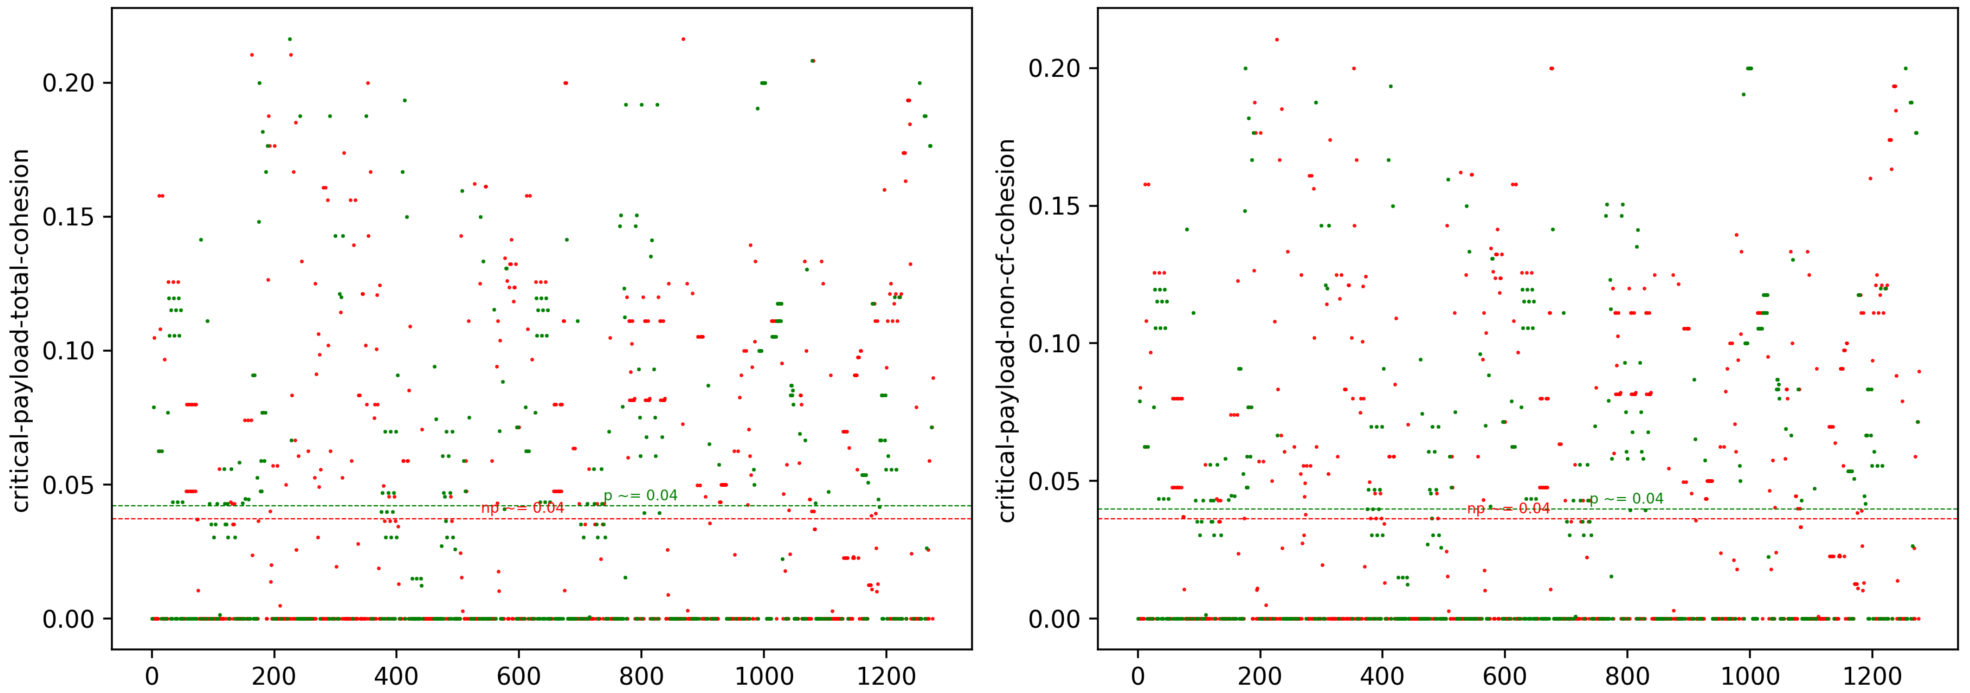
\includegraphics[width=\linewidth]{figs/loop-cohesion-0.png}
\caption{\textit{Critical payload total cohesion} metric on the left and \textit{critical payload non-cf cohesion} metric on the right. Red and green dots represent loops, which have not/have been parallelized by ICC compiler correspondingly.}
\label{loop-cohesion-0}
\end{figure}
\begin{figure}[h]
\centering
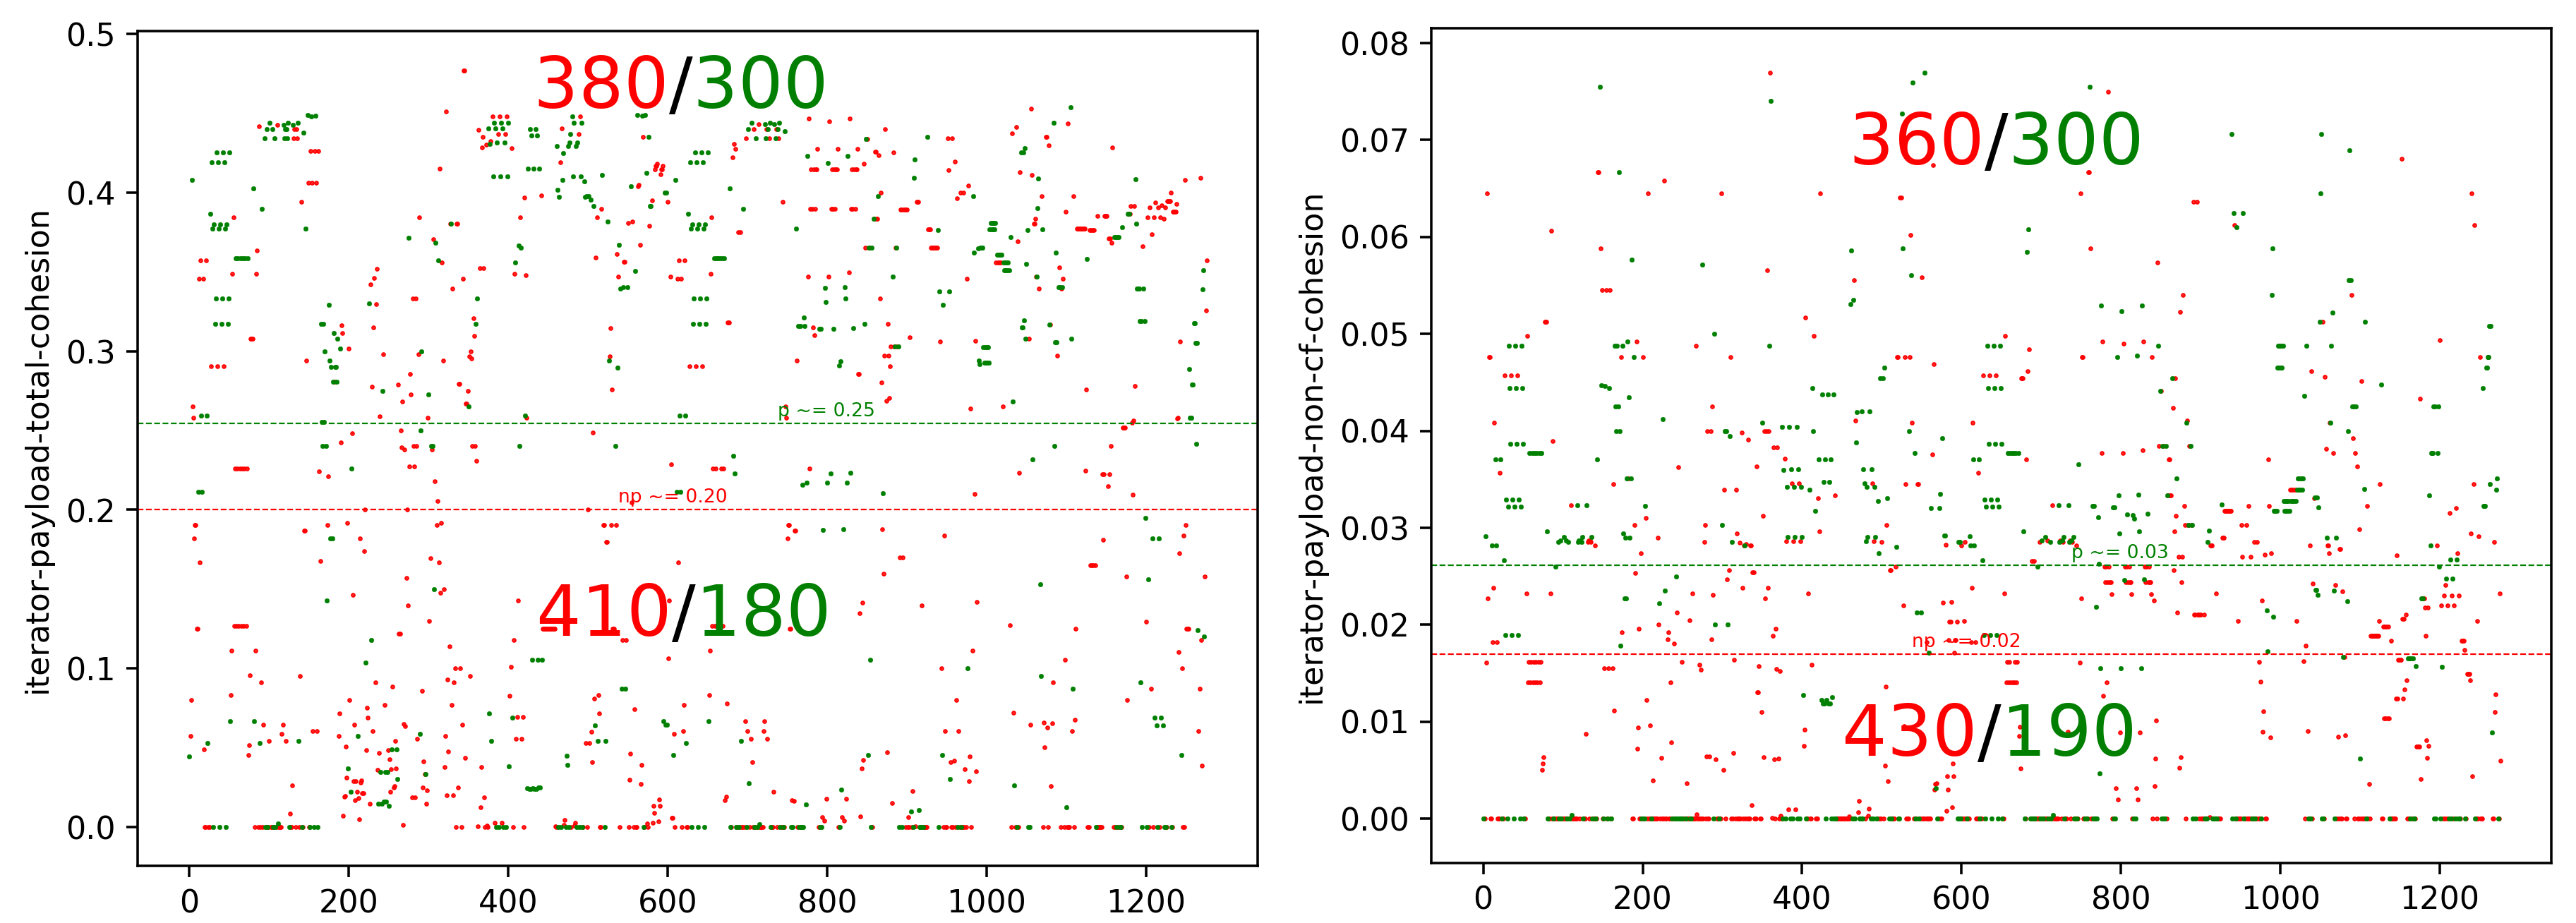
\includegraphics[width=\linewidth]{figs/loop-cohesion-1.png}
\caption{\textit{Iterator payload total cohesion} metric on the left and \textit{Iterator payload non-cf cohesion} metric on the right. Red and green dots represent loops, which have not/have been parallelized by ICC compiler correspondingly.}
\label{loop-cohesion-1}
\end{figure}
\qquad Critical payload cohesion metrics do not correlate that much with parallelizability property. Figure \ref{loop-cohesion-0} shows approximately similar mean metric values on red and green subsets and it is also visible, that red and green dots are uniformly dispersed on the plane. These cohesion metrics represent the degree of interconnection between critical part of loop payload and its non-critical part.\newline
\null\qquad On the other hand, \textit{iterator payload cohesion} metrics show a certain degree of correlation with loop parallelizability. It is visible from the two plots on figure \ref{loop-cohesion-1}, that green parallelizible dots are dispersed predominantly at the top of the plane. Mean metric values on red and green subsets tell exactly the same thing: mean metric values for parallelilazible loops tend to be higher than their counterparts on non-parallelizible subsets (0,25 versus 0,20 for \textit{iterator payload total cohesion} and 0,03 versus 0,02 for \textit{iterator payload non-cf cohesion}). Dot numbers above and below mean lines are also in inverse proportionality, as it is visible from figure \ref{loop-cohesion-1}.     
\subsection{Data clustering analysis}
\label{analysis-data-clustering-analysis}
\qquad This section describes the results of dataset clustering analysis. Data from the table \ref{analysis-data-table} can be viewed as a set of 13-dimensional vectors, describing NAS benchmark loops. These vectors map loops into 13-dimensional space. It might be interesting to see what spatial patterns and structural properties these mappings conform to. For every loop, thanks to Intel C/C++ compiler, we know the right answer regarding its parallelizability. This section reports studies about correlations between spatial and structural properties of these vector mappings and loops parallelizability.\newline
\begin{figure}[htb]
\centering
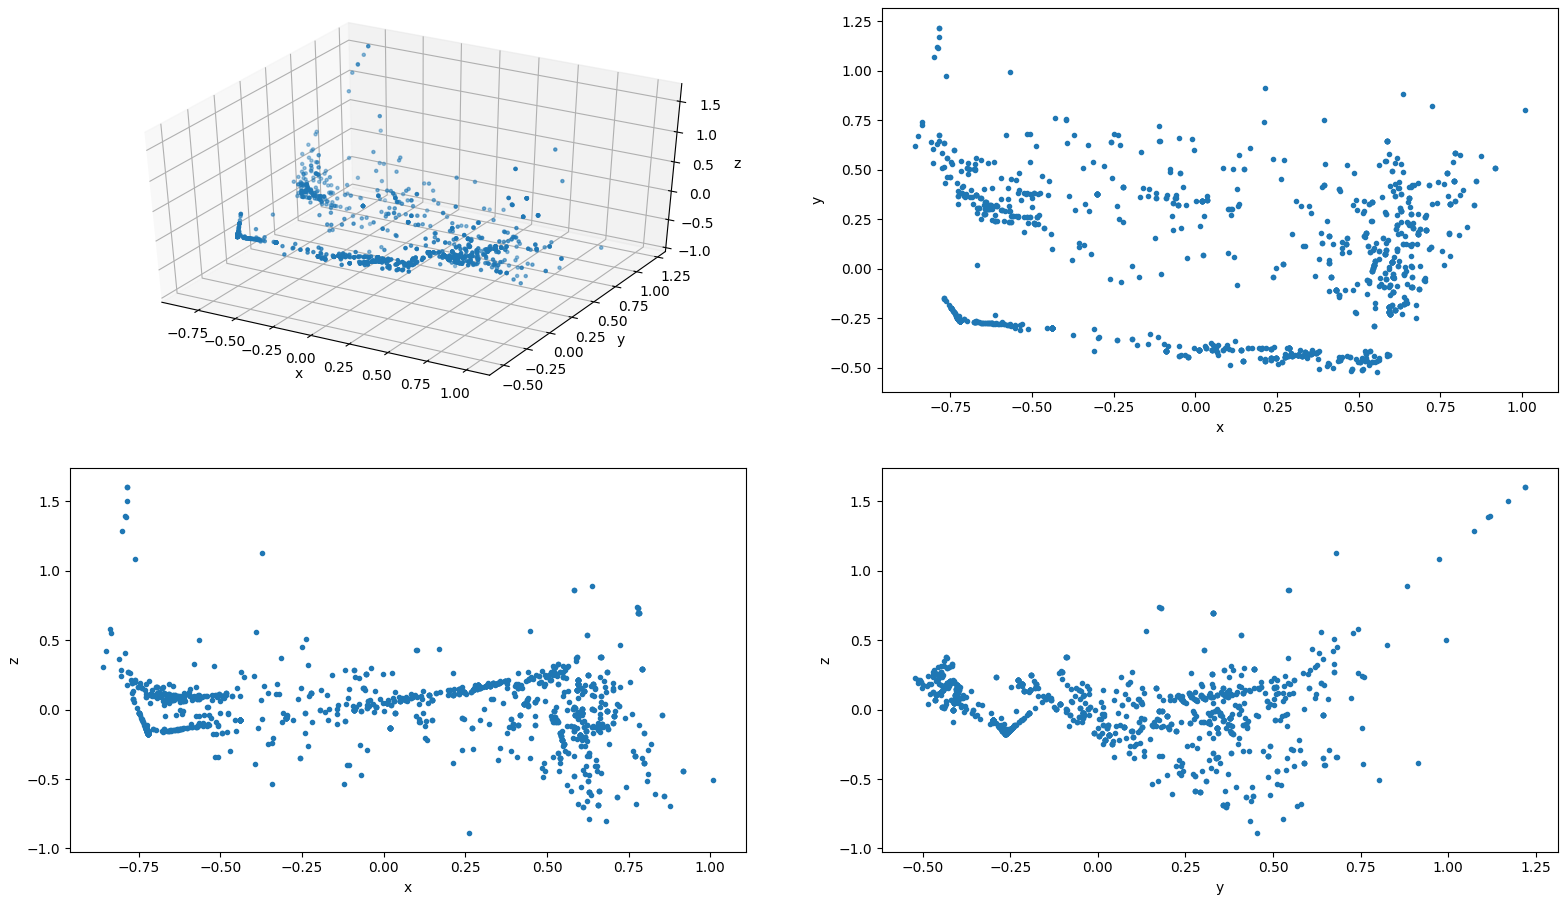
\includegraphics[width=\linewidth]{figs/metrics-pca-13-to-3.png}
\caption{Visualisation of loop metrics dataset spatial distribution (13-dimensional metric vectors have been projected onto 3D space thanks to PCA algorithm) - blue dots correspond to metric values of single loops.}
\label{metrics-pca-13-to-3}
\end{figure} \newline 
\null\qquad Since loops are represented by 13-dimensional vectors, direct dataset visualization is unfeasible. Principal Components Analysis (PCA) has been used to project the data onto 3-dimensional space and visualize it. Figure \ref{metrics-pca-13-to-3} provides an illustration of distribution of metric values on all loops. It is visible from the figure, that data values do not form any apparent clusters, but there are some areas of increased density though. Metric dataset projection onto 2D plane looks like XY projection of 3D PCA mapping (see figure \ref{metrics-pca-13-to-2}).\newline
\null\qquad Next step is to establish correlation between structural properties of dataset distribution and loop parallelizability. Figure \ref{metrics-pca-parallelizability} provides an illustration for it. Out of that figure it is visible that there is no apparent correlation between combined metric values and parallelizability of loops these metrics represent. 
\begin{figure}[htb]
\centering
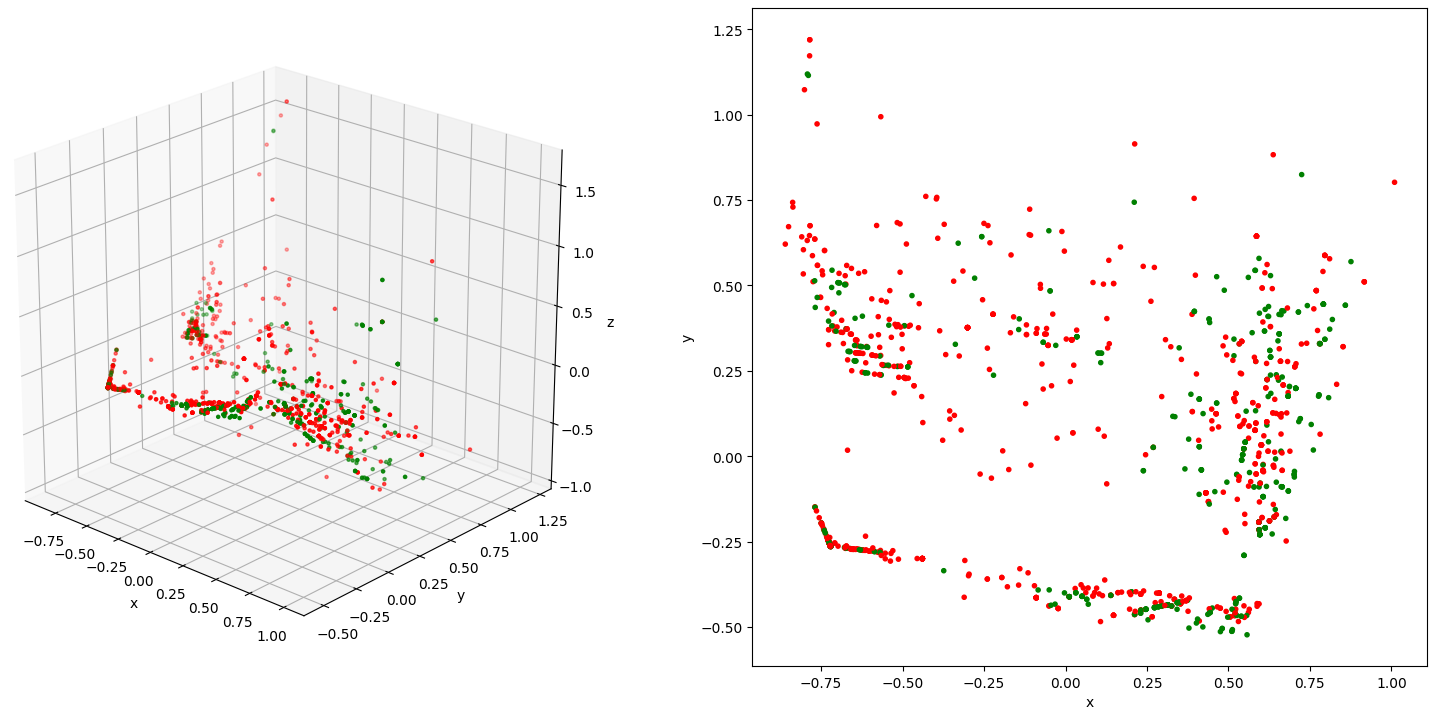
\includegraphics[width=\linewidth]{figs/metrics-pca-parallelizability.png}
\caption{Visualisation of loop metrics dataset spatial distribution (3D PCA projection on the left, 2D PCA projection on the right) versus parallelizability property. Red dots - non-parallelizible loops; green dots - parallelizible loops}
\label{metrics-pca-parallelizability}
\end{figure} \newline
\null\qquad It would be interesting to see, what kind of loops and metric values form these areas of increased density. To get that information we can apply k-means clustering algorithm and get subsets of loops, which form these condensed clots. We need to pick the number of clusters. The number of clusters might be arbitrary, but from the figure it is visible that 3 or 4 clusters would be quite a close approximation to the given dots distribution. Figure \ref{metrics-4-clusters} illustrates the results of k-means clustering algorithm run with 4 clusters. Algorithm has almost perfectly identified the structure of dots distribution. Maybe yellow and blue subsets must be in the same subset. We can consider all these blue and yellow loops altogether. Some dots (the ones on the boundary of red cluster) also happened to be blue, while red classification would be the most appropriate for them. To exclude these must-be-red blue loops from considerations applied to the blue cluster, euclidean distances from cluster centers were computed for every dot. Only loops near cluster centers are considered in the manual source code study. Table \ref{clusters-metric-values} presents average values for all metrics in 4 clusters. \newline
\begin{figure}[htb]
\centering
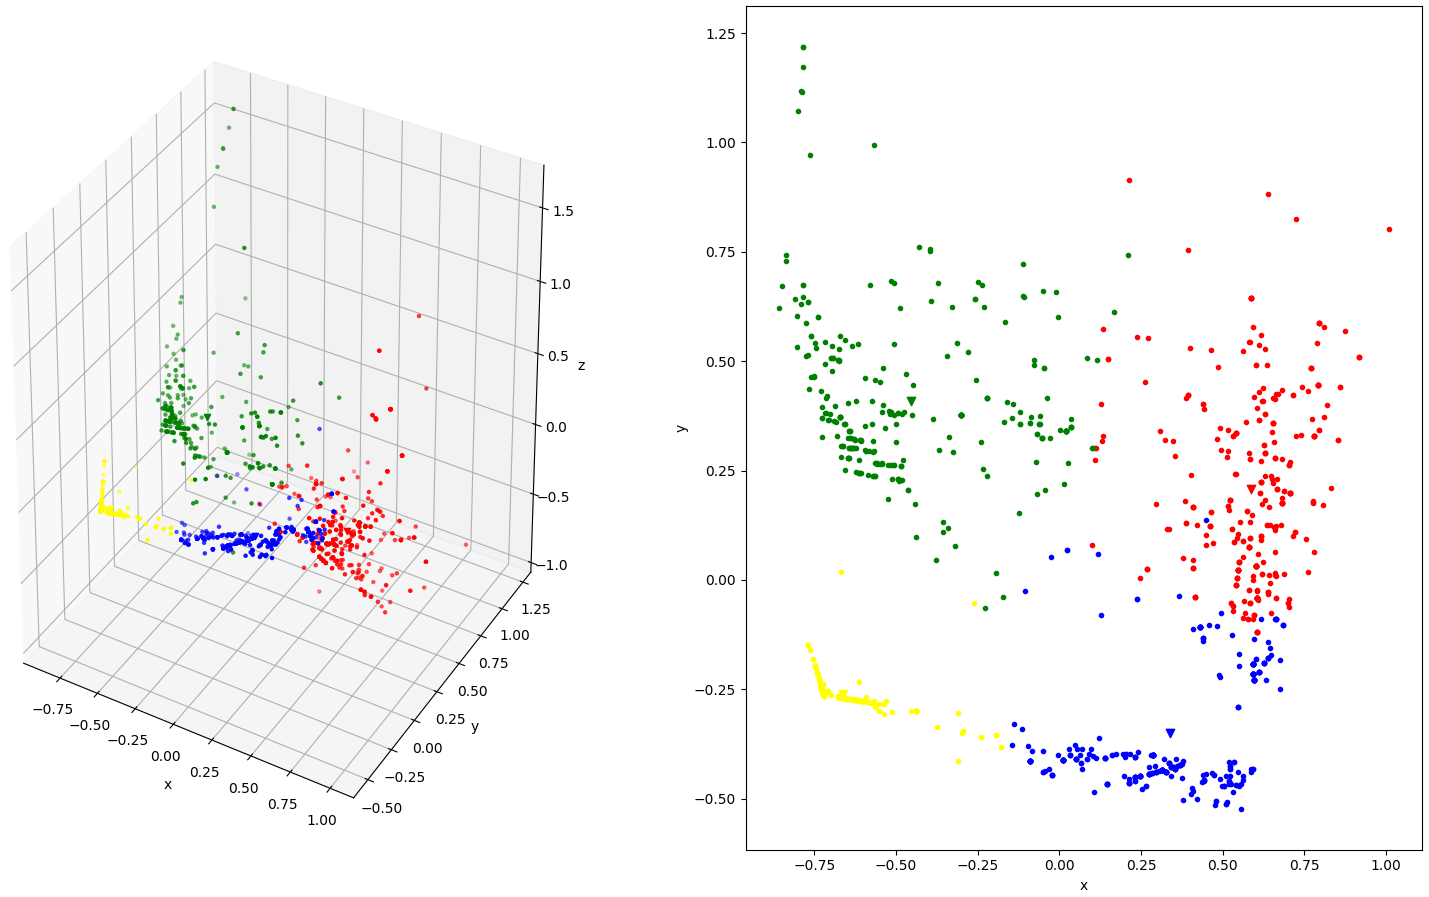
\includegraphics[width=\linewidth]{figs/metrics-4-clusters.png}
\caption{k-means algorithm classified the dataset into 4 separate clusters.}
\label{metrics-4-clusters}
\end{figure}
\begin{figure}[htb]
\centering
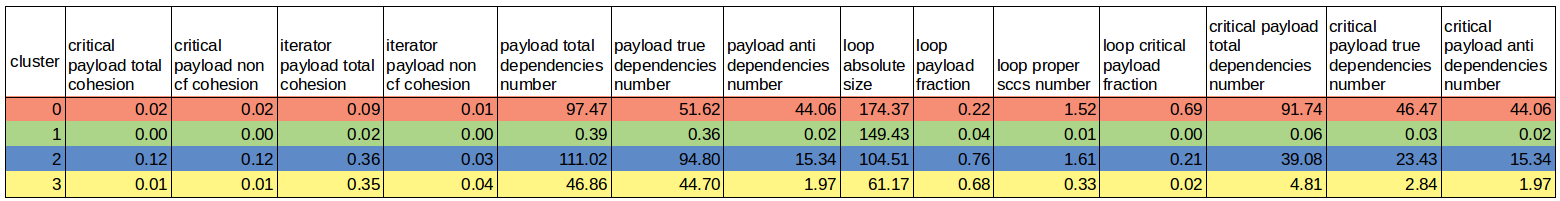
\includegraphics[width=\linewidth]{figs/clusters-metric-values.png}
\caption{Average metric values for 4 different clusters}
\label{clusters-metric-values}
\end{figure} \newline 
\null\qquad Out of that table \ref{clusters-metric-values} and figure \ref{metrics-4-clusters} we can derive metric growth directions. All critical payload part related metrics show tendency to grow anti-clockwise, having minimum values in the green dot cluster and maximum values in the red one. We can combine all these metrics in one \textit{critical component size} characteristic. Cohesion between loop iterator and payload parts grows from green cluster towards all 3 other clusters, reaching its maximum values in blue and yellow clusters. \textit{Loop absolute size} has a mirrored (in relation to \textit{iterator payload cohesion} metric) pattern of growth. It starts to grow in the yellow cluster and takes on higher values as it reaches 3 other clusters. Figure \ref{clusters-metric-values} presents the final illustration for all considerations above.\newline   
\begin{figure}[htb]
\centering
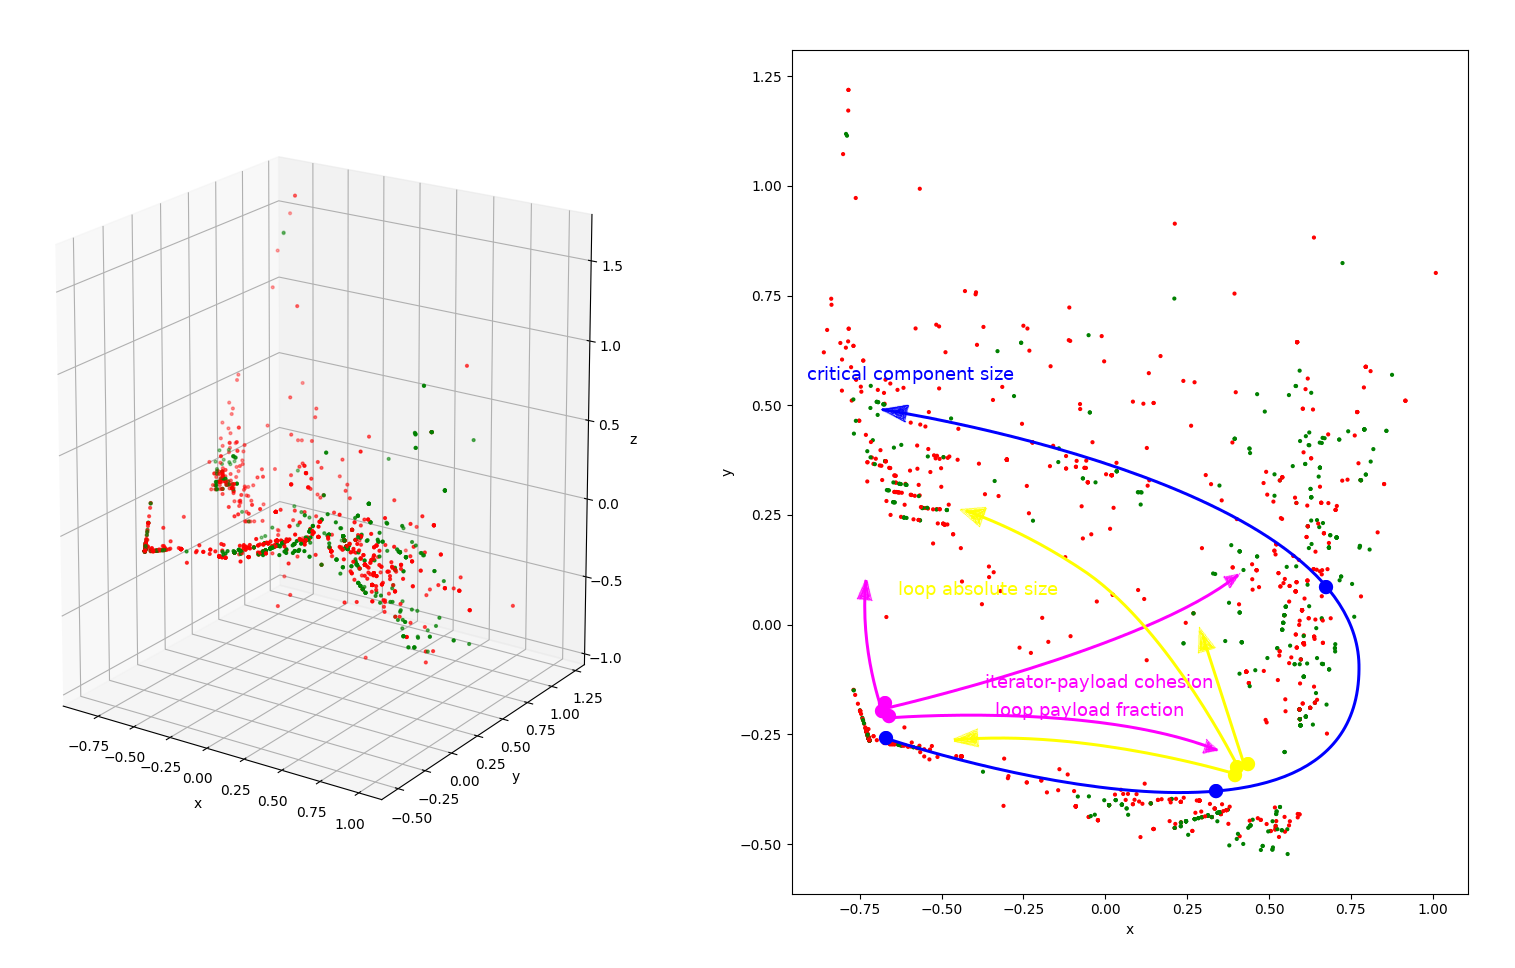
\includegraphics[width=\linewidth]{figs/metrics-growth-directions.png}
\caption{Correspondence between 3D PCA projected distribution and original metric values, set by growth arrowed lines.}
\label{clusters-metric-values}
\end{figure}\newline
\null\qquad The next section \ref{analysis-manual-analysis} provides examples of loops, which can be found in these 4 built clusters.  

\subsection{Decision tree based parallelisability classification}
\qquad Decision tree is another human-comprehensible dataset visualization technique. Figure \ref{decision-tree-depth-3} has been produced with scikit-learn \cite{python-lib-scikit-learn} decision tree classifier and represents a decision tree learned from metrics table dataset \ref{analysis-data-table}. Decision tree sorts metric vectors down the tree. Sorting starts from the root and goes along all the sorting rules down to the leaf. Leaf provides the final metric vector classification. For simplicity and feasibility of visualisation, the depth of the tree has been limited to 3. This limitation leads to some probabilistic errors in the final loop parallelizability classification, but is still capable of capturing the main trends in the data. \ref{analysis-data-table}.\newline
\null\qquad The construction of decision tree is based on the notions of entropy and information gain. Decision tree algorithm finds and places in the root of the tree a rule, which separates the dataset in a way, that brings the biggest information gain (in other words, decreases entropy of the dataset the most). Then it goes along all the branches down the tree and places the most information gaining rule at every node, calculated on the dataset subset, corresponding to that node.\newline
\null\qquad As we can see from the figure \ref{decision-tree-depth-3}, scikit-learn implementation of decision tree algorithm picked \textit{iterator-payload non-cf cohesion} as a metric, separating the input dataset in the best way. The input dataset contains 1277 metric vectors, 790 of them are classified as non-parallelizible and 487 as parallelizible. The entropy of such a dataset equals to $S=-\frac{790}{1277}\cdot \log_{2}\frac{790}{1277}-\frac{487}{1277}\cdot \log_{2}\frac{487}{1277}\approx 0.96$. After the rule in the root split the dataset into two subsets, corresponding to the left and right subtrees, the entropy became $S=\frac{790}{1277}\cdot S_{True} + \frac{487}{1277}\cdot S_{False} = \frac{793}{1277}\cdot (-\frac{591}{793}\cdot \log_{2}\frac{591}{793}-\frac{202}{793}\cdot \log_{2}\frac{202}{793}) + \frac{484}{1277}\cdot (-\frac{199}{484}\cdot \log_{2}\frac{199}{484}-\frac{285}{484}\cdot \log_{2}\frac{285}{484})\approx $.     
\begin{figure}[htb]
\centering
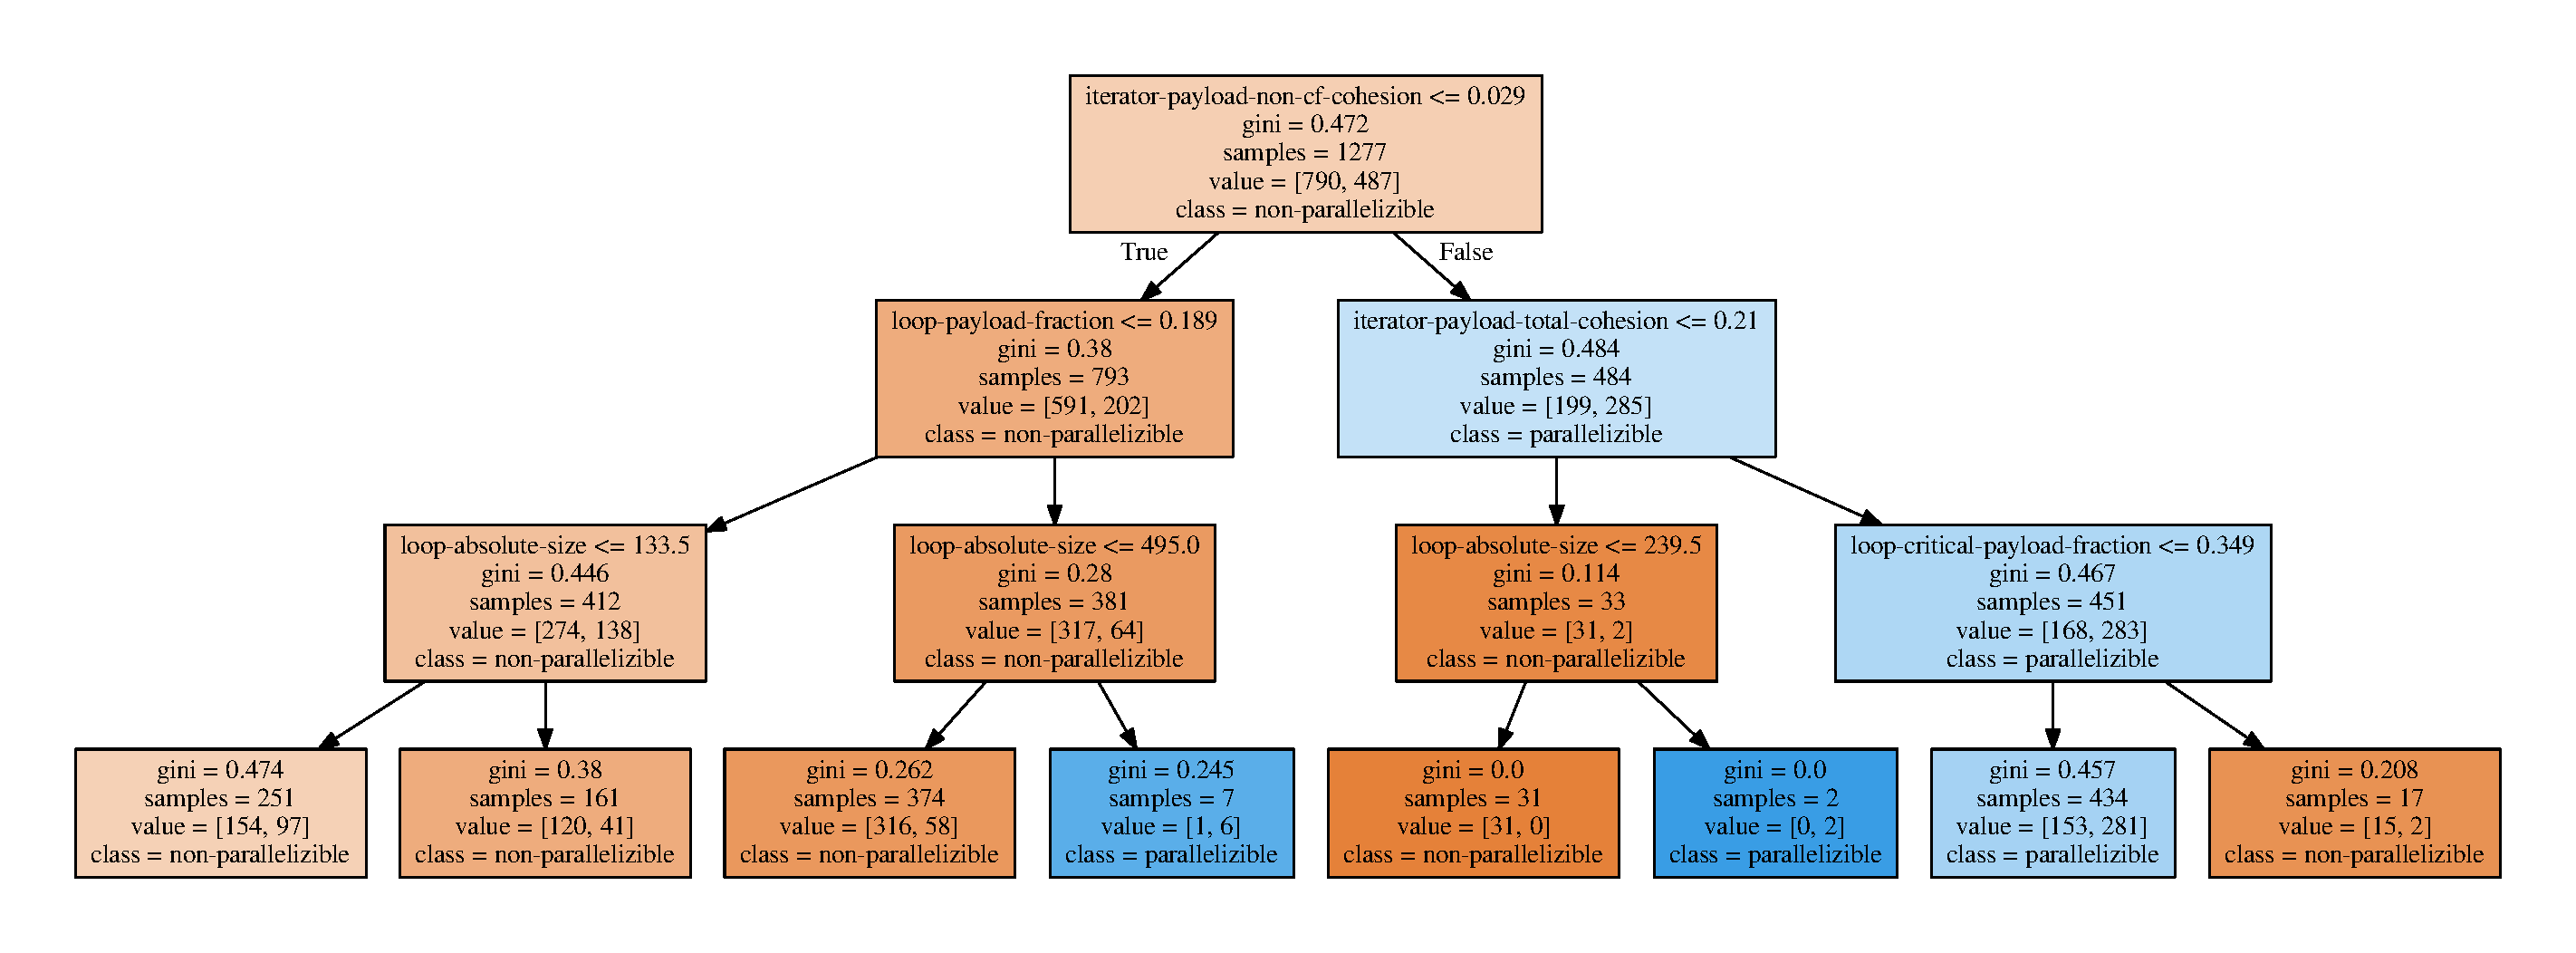
\includegraphics[width=\linewidth]{figs/decision-tree-depth-3.pdf}
\caption{Dataset \ref{analysis-data-table} decision tree, limited to the depth of 3.}
\label{decision-tree-depth-3}
\end{figure}\newline
\null\qquad For the purpose of our work we can interpret that decision tree in the following way. If we use \textit{iterator-payload non-cf cohesion} metric to judge about loop parallelizability, then we should compare the value of that metric for a loop being considered against 0,03. If the value on the loop is grater than 0,03, then the loop is parallelizible with probability of $\frac{285}{484}\approx 60\%$ and non-parallelizible with probability of $\frac{199}{484}\approx 40\%$. That numbers do not give us a lot of information, but if value of the metric on a loop happens to be below 0,03, then the loop is most likely to be non-parallelizible with probability of $\frac{591}{793}\approx 75\%$. The latter signals loop code developer to reconsider his code, if he wants his code to take advantage of parallelization.\newline 
\null\qquad These are basically the same results as ones in the section \ref{analysis-single-metrics-vs-parallelizability} of the current chapter, but decision tree methods have more solid mathematical grounds and foundation. Decision tree algorithm automatically finds a decision boundary in the range of single metric values, that splits the dataset in the most information gaining way. The tree on the figure \ref{decision-tree-depth-3} has been built from the set of all 13 metrics. According to the algorithm criteria \textit{iterator-payload non-cf cohesion} metric is the best for loop parallelizability analysis task. If we exclude that metric from the set of metrics for the root rule search, or even use just one metric, we can find decision boundaries with corresponding probabilities for all more or less parallelizability correlating metrics. Figure \ref{decision-trees-single-metrics} shows the result.
\begin{figure}[htb]
\centering
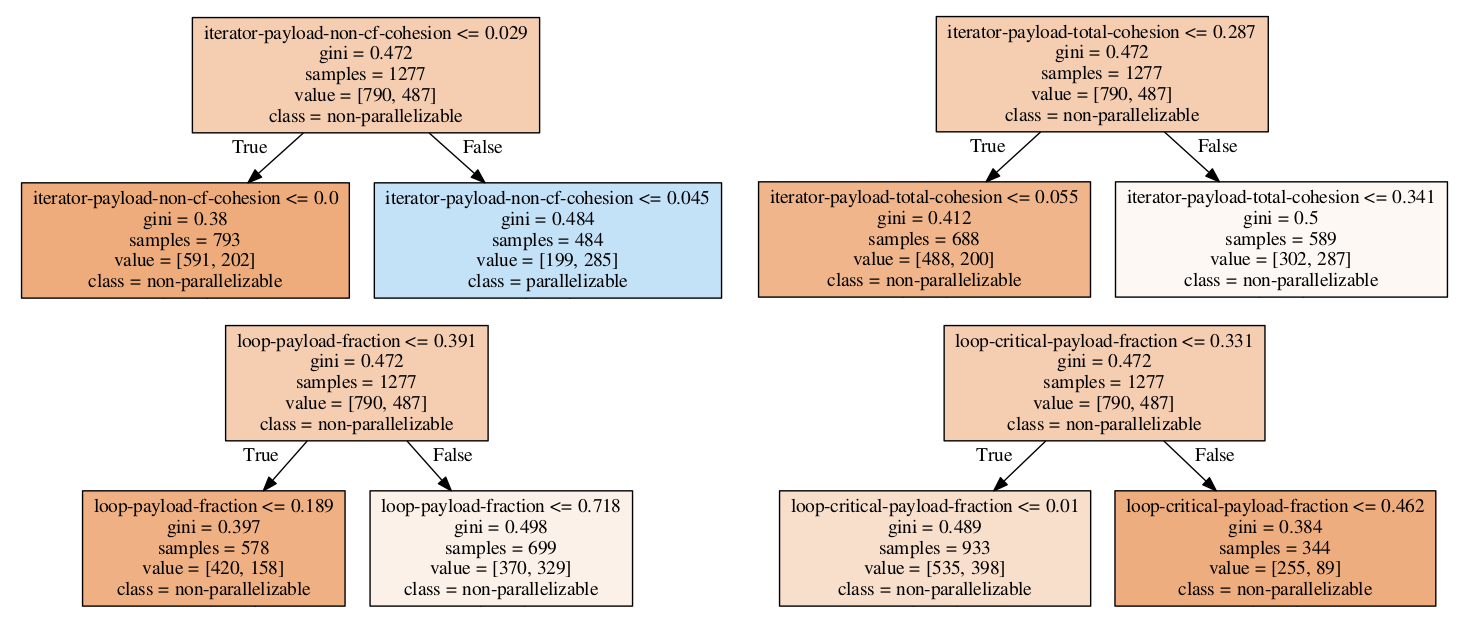
\includegraphics[width=\linewidth]{figs/decision-trees-single-metrics.png}
\caption{Decision boundaries and corresponding parallelizable/non-parallelizable probabilities for the best corerlating single metrics.}
\label{decision-trees-single-metrics}
\end{figure}\newline
\null\qquad We can see from the above figure \ref{decision-trees-single-metrics}, that if we use \textit{iterator-payload total cohesion} as a root node instead, we are going to get 0,287 decision boundary with 70\% non-parallelizible and 30\% parallelizible below 0,287 and 41\% non-parallelizible and 59\% parallelizible above the boundary. So, \textit{iterator-payload total cohesion} is slightly worse than \textit{iterator-payload non-cf cohesion}. It makes sence, since most iterators have control-flow structures, controlling conditions of the loop, but true dependencies are usually introduced by data edges from iterator to the payload. Metric \textit{loop critical payload fraction} can be used in the inverse way. If the value of this metric for a given loop happens to be greater than 0,33 decision boundary, then this loop is 74\% non-parallelizible. The latter result correlates with the common sense: the bigger critical payload part of the loop, the harder this loop is for dependence breaking and parallelization. The last metric in the figure \ref{decision-trees-single-metrics} is \textit{loop payload fraction}. We can see that the decision boundary for that metric is 0.391. So, if the payload of the loop happes to be less than 40\% of the total loop size, then this loop most likely is non-parallelizible with corresponding probability of approximately 73\%. That also makes sense, since big iterators include too much computations in them, which makes such loops hard to parallelize. Computations should be concentrated in the payload of the loop and iterators should be relatively simple.\newline
\null\qquad We don't necesserily need to use only single metrics. For a given loop we can compute a set of metrics and walk with their corresponding values down the decision tree in the figure \ref{decision-tree-depth-3}, which has been taught by parallelizible Intel C/C++ compiler. Use of multiple features increases the accuracy of results. For example, lets look at the figure \ref{decision-tree-depth-3}. Once we checked a loop being examing against the first root node rule and identified that the \textit{iterator-payload non-cf cohesion} metric happened to be greater than 0,03 decision boundary, we can check the second rule, namely $\textit{iterator-payload non-cf cohesion}\leq 0,21$. If we go along the blue (parallelizible) boxes, than we get $\frac{281}{434}\approx 65\%$ parallelizability chance against 59\% after only \textit{iterator-payload non-cf cohesion} boundary check. While parallelizability probabilities may not seem big enough for being worth the analysis, non-parallelizability probability in the left subtree can reach 85\% for a relatively big (374 samples) subset. For getting that estimate, metric values on a loop must satisfy to a system of 3 inequalities:\newline
\begin{equation*}
\begin{cases}
\begin{aligned}
\textit{iterator-payload non-cf cohesion}            &\le 0,029 \\[1ex]
\textit{loop payload fraction} &\le 0.189 \\[1ex]
\textit{loop absolute size} &\leq 495
\end{aligned}
\end{cases}
\end{equation*}\newline
\null\qquad If we limit the depth of decision tree to 5 instead of 3, decision tree algorithm is going to add less parallelizability correlating metrics to consideration as well. Non-parallelizible predictions are not that interesting as parallelizable. Decision tree of depth 5 can predict parallelizability with better probabilities. For example, the two systems of inequalities below are going to conclude that a given loop is $\frac{207}{322}\approx 64\%$ and $\frac{56}{61}\approx 92\%$ parallelizable correspondingly.\newline
\null\qquad It would be of special interest to take a look at loops, which satisfy all these inequalitis, but nonetheless end up to be non-parallelizible. Such loops have not been parallelized by Intel ICC compiler, but have been classified as parallelizible by the set of metrics. If there are any among these loops, that are algorithmically parallel, but have not been parallelized by Intel compiler due to some lower-level technical issues, then these metrics find to be quite useful by telling software developed, that he should not listen to Intel compiler and take a closer human look at them. Section conducts such an analysis.
\begin{equation*}
\begin{cases}
\begin{aligned}
\textit{iterator-payload non-cf cohesion}            &\le 0,029 \\[1ex]
\textit{iterator-payload total cohesion} &\leq 0,21 \\[1ex]
\textit{loop critical payload fraction} &\leq 0,349 \\[1ex]
\textit{loop proper SCCs number} &\leq 1,5 \\[1ex]
\textit{critical payload true dependencies number} &\leq 6,5
\end{aligned}
\end{cases}
\end{equation*}\newline
\begin{equation*}
\begin{cases}
\begin{aligned}
\textit{iterator-payload non-cf cohesion}            &\le 0,029 \\[1ex]
\textit{iterator-payload total cohesion} &\leq 0,21 \\[1ex]
\textit{loop critical payload fraction} &\leq 0,349 \\[1ex]
\textit{loop proper SCCs number} &\leq 1,5 \\[1ex]
\textit{loop payload fraction} &\leq 0,575
\end{aligned}
\end{cases}
\end{equation*}\newline
    
\section{Manual analysis}
\label{analysis-manual-analysis}
\qquad Let's start from a trivial case and consider a loop, presented in listing \ref{lst:non-parallel-0}. This loop fills timer records array \textit{trecs[]} with timer reads. The latter are computed inside \textit{timer\_read()} function. Intel C/C++ compiler has to be conservative and does not parallelize that function, since it is not clear, whether there is a cross-iteration dependency introduced from inside the function, but the decision tree, presented in the figure \ref{decision-tree-depth-3} classifies that loop as parallelizible. Given that hint a programmer might check, if there are actually any states, preserved by \textit{timer\_read()} function from call to call, which might be distorted by the loop parallelization. This loop has \textit{iterator payload non-cf cohesion} equal to 0.0645, which correspond to parallelizible loops, according to results presented in the section \ref{analysis-single-metrics-vs-parallelizability}.              
\begin{lstlisting}[caption={Loop, which has not been parallelized by Intel C/C++ compiler, but does seem algorithmically parallelizible, given absense of cross-iteration dependencies introduced by the function call. }, captionpos=b, label=lst:non-parallel-0, float,floatplacement=H]
for (i = 1; i <= t_last; i++) {
	trecs[i] = timer_read(i);
}
\end{lstlisting}\newline
\null\qquad Another more elaborate case is presented in the listing \ref{lst:non-parallel-1}. Intel compiler failed to parallelize that loop nest, because it assumed that there is flow and anti dependencies between load from rhs[k][j][i][m] and store to rms[m]. But decision tree of depth 3 (see figure \ref{decision-tree-depth-3}) classifies that innermost loop as 65\% parallelizible and 35\% not, giving a programmer a little hope. Its classification could have been slightly better if there was not SCC inside the payload of the inner loop. Metric computing pass uses LLVM memory dependence analysis, which alike Intel compiler assumes dependencies between memory references to different arrays. Metric values for the innermost loop are: $\textit{iterator-payload non-cf cohesion}\approx 0.0357$, $\textit{iterator-payload total cohesion}\approx 0.3571$, $\textit{loop critical payload fraction}\approx 0.2963$.
\begin{lstlisting}[caption={\textit{SNU\_NAS/BT/src/error.c:84}. Loop, which has not been parallelized by Intel C/C++ compiler due to conservative anti and flow dependencies assumptions between references to rhs and rms. But these are different arrays and the loop actually computes reduction.}, captionpos=b, label=lst:non-parallel-1, float,floatplacement=H]
for (k = 1; k <= grid_points[2]-2; k++) {
	for (j = 1; j <= grid_points[1]-2; j++) {
		for (i = 1; i <= grid_points[0]-2; i++) {
			for (m = 0; m < 5; m++) {
				add = rhs[k][j][i][m];
				rms[m] = rms[m] + add*add;
			} 
		} 
	} 
}
\end{lstlisting}\newline
\null\qquad Assuming that a programmer accepted that metric hint, he decided to analyze and rewrite the loop with OpenMP pragmas (see figure \ref{lst:non-parallel-2}), since it it visible, that the loop computes reductions for all 5 rms array elements \ref{eq:equation-0}:\newline
\begin{equation}
rms\left[ m \right] = \sum\limits_{k \in grid\_points\left[ 2\right] -2}\sum\limits_{j \in grid\_points\left[ 1\right] -2}\sum\limits_{i \in grid\_points\left[ 0\right] -2} rhs\left[ k\right] \left[ j\right] \left[ i\right] \left[ m\right]
\label{eq:equation-0}
\end{equation}
\begin{lstlisting}[caption={Loop, which has not been parallelized by Intel C/C++ compiler, but does seem algorithmically parallelizible, given absense of cross-iteration dependencies introduced by the function call. }, captionpos=b, label=lst:non-parallel-2, float,floatplacement=H]
#pragma omp for nowait
for (k = 1; k <= grid_points[2]-2; k++) {
	for (j = 1; j <= grid_points[1]-2; j++) {
		for (i = 1; i <= grid_points[0]-2; i++) {
			for (m = 0; m < 5; m++) {
				add = rhs[k][j][i][m];
				rms_local[m] = rms_local[m] + add*add;
			} 
		} 
	} 
} 
for (m = 0; m < 5; m++) {
#pragma omp atomic
	rms[m] += rms_local[m];
}
\end{lstlisting}
\null\qquad Let's consider some more examples. Listing \ref{lst:non-parallel-3} shows another loop example, which computes reduction \ref{eq:equation-1}.
\begin{equation}
key\_buff\_ptr\left[ i \right] = \sum\limits_{j=0}^{i-1} key\_buff\_ptr\left[ i\right]
\label{eq:equation-1}
\end{equation}
\null\qquad It is clear, that the loop in listing \ref{lst:non-parallel-3} should be rewritten in order to be parallelizible, but Intel compiler gives just answer "no", but programmer takes a look at the values of metrics: \textit{iterator-payload-non-cf-cohesion}: 0.04, \textit{iterator-payload-total-cohesion}: 0.3, \textit{loop-critical-payload-fraction}: 0.3077. These values take the loop down the decision tree \ref{decision-tree-depth-3} into parallelizible classification. Programmer might take that hint and rewrite the loop.\newline
\begin{lstlisting}[caption={\textit{SNU\_NAS/IS/is.c:508}. Algorithmically parallelizible problem ends up hidden from compiler behind unsuccessful implementation.}, captionpos=b, label=lst:non-parallel-3, float, floatplacement=H, mathescape=true]
for( i=0; i<MAX_KEY-1; i++ ) {
	key_buff_ptr[i+1] += key_buff_ptr[i];
}
\end{lstlisting}
\null\qquad NAS benchmarks contain a lot of such examples. Listings \ref{lst:non-parallel-4}, \ref{lst:non-parallel-5} show some more of them.

\begin{lstlisting}[caption={\textit{SNU\_NAS/IS/is.c:468}. Algorithmically parallelizible problem ends up hidden from compiler behind unsuccessful implementation. Metrics: \textit{iterator-payload-non-cf-cohesion}: 0.0566, \textit{iterator-payload-total-cohesion}: 0.3208, \textit{loop-critical-payload-fraction}: 0.2143, \textit{loop-payload-fraction}: 0.6087}, captionpos=b, label=lst:non-parallel-4, float, floatplacement=H, mathescape=true]    
for( i=1; i< NUM_BUCKETS; i++ ) {  
	bucket_ptrs[i] = bucket_ptrs[i-1] + bucket_size[i-1];
}
\end{lstlisting}

\begin{lstlisting}[caption={\textit{SNU\_NAS/LU/src/l2norm.c:57}. Intel compiler refuses to parallelize that reduction problem due to assumed true and anti dependencies between memory references to different sum and v arrays. Inner loop metrics: \textit{iterator-payload-non-cf-cohesion}: 0.0331, \textit{iterator-payload-total-cohesion}: 0.3967, \textit{loop-critical-payload-fraction}: 0.1364, \textit{loop-payload-fraction}: 0.8148}, captionpos=b, label=lst:non-parallel-5, float, floatplacement=H, mathescape=true] 
for (k = 1; k < nz0-1; k++) {
	for (j = jst; j < jend; j++) {
		for (i = ist; i < iend; i++) {
			for (m = 0; m < 5; m++) {
				sum[m] = sum[m] + 
					v[k][j][i][m] * v[k][j][i][m];
			}
		}
	}
}
\end{lstlisting}

\section{Statistical analysis}
\label{analysis-statistical-analysis}
\qquad Statistical learning techniques can be used to compare relative performance of software source code metrics in the task of parallelizability classification. This section views loop parallelizability as a machine learning problem. Metrics represent features of loops. Intel C/C++ compiler gives an expert-opinion and labels (classifies) loops as parallelizible or not. Three ML algorithms have been applied to the dataset presented in figure \ref{analysis-data-table}: Support Vector Machines (SVM), decision tree classifier, neural network based Multi-layer Perceptron (MLP). All machine learning metric set studies have been conducted with the help of pandas \cite{python-lib-pandas} and scikit-learn \cite{python-lib-scikit-learn} python packages. Detailed description of all algorithms, techniques and all underlying mathematical foundations can be found in the introduction to statistical analysis book \cite{statistical-learning-book}.\newline
\null\qquad Table \ref{single-metric-ml-table-0} below presents results obtained for every single loop parallelizability metric out of proposed metric set (see section \ref{metrics-metric-groups}).
\begin{figure}[htb]
\centering
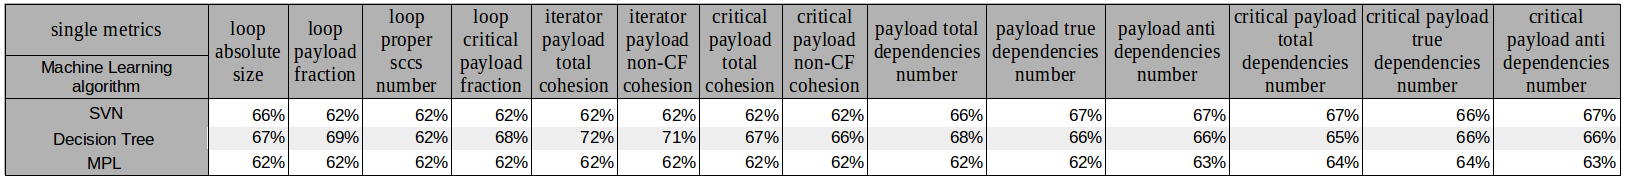
\includegraphics[width=\linewidth]{figs/single-metric-ml-table-0.png}
\caption{Average accuracies of parallelizability predictors. Each predictor has been trained with only one feature (table columns). Different machine learning techniques (SVN, Decision Tree, MPL) have been used for training. Percentages in the table represent mean accuracies. K-fold (K=15) cross validation technique has been used to partition samples from \ref{analysis-data-table} into training and testing sets. Different K numbers (5, 10, 20, 30) produce approximately the same mean accuracies (see figure \ref{single-metric-ml-table-1}).}
\label{single-metric-ml-table-0}
\end{figure}\newline 
\null\qquad Every single metric has been used as a loop feature, to train different machine learning models to classify loops as parallelizible or not. Above table \ref{single-metric-ml-table-0} reports on accuracies of corresponding trained predictor models. In order to train every single model, the dataset \ref{analysis-data-table} has been partitioned into training and testing subsets. Partitioning has been done with K-fold method. This method splits all data samples into K equal subsets. Then it chooses one of these spilts as a testing set and uses all the rest as a training set. This process is repeated K times to cover all possible cases. Then K-fold partitioning might be applied again, but with different partitions. That application might be repeated N times. For the table \ref{single-metric-ml-table-0} above K=15, N=5. For every training and testing run predictors report accuracy. All these accuracies have been averaged to just one percentage, presented in the table \ref{single-metric-ml-table-0} above.\newline
\null\qquad Exactly the same experiment (with K=15 and N=5) has been conducted with different sets of metrics used as features of predictor models. Table \ref{metric-set-ml-table-0} below shows collected results.
\begin{figure}[htb]
\centering
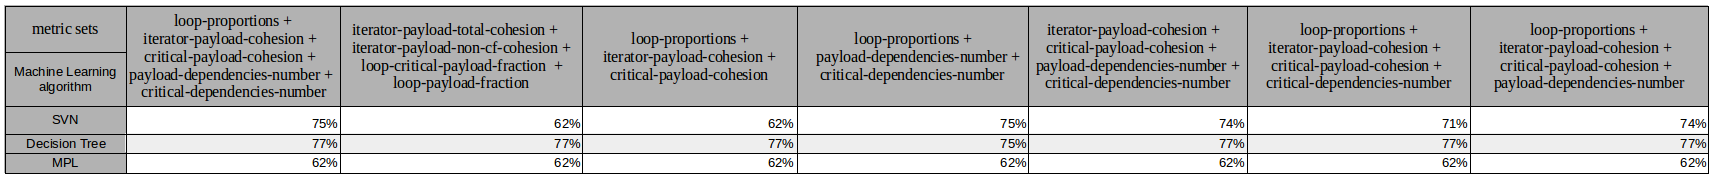
\includegraphics[width=\linewidth]{figs/metric-set-ml-table-0.png}
\caption{Average accuracies of parallelizability predictors. Each predictor has been trained from sets of metrics. Results are presented in the same form as in table \ref{single-metric-ml-table-0} above. Full table, with all K values (5,10,15,20,30) is available in the figure \ref{metric-set-ml-table-1} in the appendix.}
\label{metric-set-ml-table-0}
\end{figure}\newline
\null\qquad Results, presented in tables \ref{single-metric-ml-table-0} and \ref{metric-set-ml-table-0} do not change significantly with K and N variations. Corresponding tables \ref{single-metric-ml-table-1} and \ref{metric-set-ml-table-1} in the appendix show the whole sets of accuracies for K equal to 5, 10, 15, 20 and 30.\newline
\null\qquad It is visible from the tables, that decision tree learning method works the best in both cases: for models with single loop metrics as featues, as well as for models with sets of metrics as features. For models with single metrics as features, decision tree makes predictions with accuracy around 65-70\%, with 71-72\% for two \textit{iterator payload cohesion} metrics. These metrics seem to work a bit better than others, what corerlates with conclusions made in section \ref{analysis-single-metrics-vs-parallelizability} of this chapter.\newline
\null\qquad When we use sets of metrics as machine learning model features, accuracies these machine learning predictors can achieve are a bit higher. Decision tree based algorithm can achieve accuracy of 77\%. This learning algorithm works comparably for all sets. For the set in the first column of table \ref{metric-set-ml-table-0} (with all 13 metrics out of 5 groups used as features) decision tree works as good as for the set in the second column (just 4 most parallelizability correlating metrics). On the other hand, accuracies of SVN based model tend to be noticably higher for models with more metrics as features. Table \ref{metric-set-ml-table-0} shows, that when we add dependencies number metrics to feature sets we get increaced prediction accuracy. It might look weird in the light of absence of any correlations between dependencies number metrics and loop parallelizability, as was shown in the section \ref{analysis-single-metrics-vs-parallelizability}. \textit{Loop proportion} metrics combined with \textit{loop cohision} metrics tend to work much worse, than \textit{loop proportion} metrics combined with \textit{loop dependencies} number metrics. This result is also a bit surprising, because \textit{loop cohesion} metrics correlate with parallelizability better, that \textit{loop dependencies number} metrics.\newline
\null\qquad Results of decision tree learning algorithm corelate better with the results presented in section \ref{analysis-single-metrics-vs-parallelizability} of this chapter, than SVN results. MPL accuracies do not seem to change with different feature sets at all.  
          